
\chapter{Begriffe}
\section{IT-Sicherheit: Ziele}
\begin{itemize}
	\item \textbf{Vertraulichkeit:} Zugriff auf autorisierte Personen begrenzt.
	\item \textbf{Integrität:} Informationen nur von autorisierten Personen veränderbar.
	\item \textbf{Verfügbarkeit:} Autorisierte Personen können auf die Informationen zugreifen, wenn benötigt.
\end{itemize}

\section{IT-Sicherheit: optionale Ziele}
\begin{itemize}
	\item \textbf{Auditierbarkeit:} Sicherheitsrelevante Eigenschaften einsehbar und überprüfbar.
	\item \textbf{Non-Repudation:} Aktionen am System nicht abstreitbar.
	\item \textbf{Accountability:} Änderungen am System immer einer Person zuzuordnen.
	\item \textbf{Privacy:} Personenbezogene Daten werden geschützt.
	\item \textbf{Authentizität:} Informationen einem bestimmten Sender zuzuordnen.
	\item \textbf{Deniability:} Inhalte oder Beiteilung einer Kommunikation im Nachhinein nicht nachweisbar.
\end{itemize}
\begin{figure}[H]
	\begin{center}
		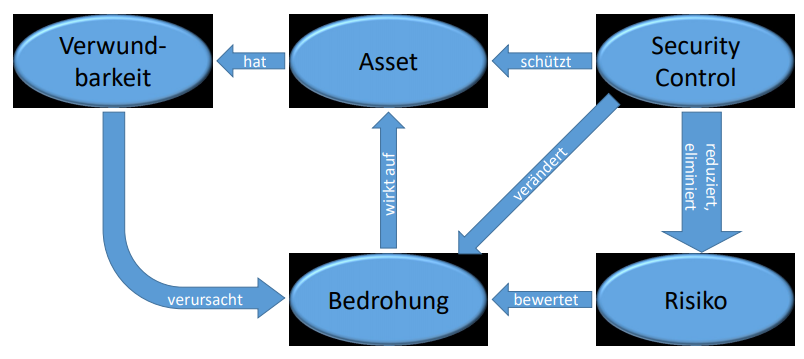
\includegraphics[scale=0.5]{Resources/Grundbegriffe.png}
		\caption{}
		\label{fig:Grundbegriffe}
	\end{center}
\end{figure}

\paragraph{Asset}
\begin{itemize}
	\item Ressource, Prozess, Produkt oder System
	\item besitzt \textbf{Wert} für die Organisation
	\item muss \textbf{geschützt} werden
\end{itemize}

\paragraph{Bedrohung}
\begin{itemize}
	\item kann \textbf{unerwünschten} Effekt haben (schädlich)
	\item \textbf{Ursachen in der Umwelt} (Überschwemmung, Feuer)
	\item \textbf{Von Menschen verursacht} (Fehler oder Vorstatz)
\end{itemize}

\paragraph{Verwundbarkeit}
fehlender, oder schwacher Schutz eines Assets. Verursacht, dass Bedrohung:
\begin{itemize}
	\item auftritt
	\item mit höherer Wahrscheinlichkeit oder Häufigkeit auftritt
	\item einen höheren Schaden verursacht
\end{itemize}

\paragraph{Risiko} Kombination aus Wahrscheinlichkeit und Auswirkungen einer Bedrohung.\\
$R_{Thread} = P_{Thread} \times D_{Thread}$\\
$P_{Thread} = Eintrittswahrscheinlichkeit$\\
$D_{Thread} = Schaden$\\
\textbf{Risikobewertung} qualitativ oder quantitativ.

\paragraph{Security Control}
\begin{itemize}
	\item \textbf{Deterrent Control:} Verringert $P_{Thread}$
	\item \textbf{Preventative Control:} Eliminierung des Risikos durch entfernen der Schwachstelle.
	\item \textbf{Detective Control:} Erkennung der Bedrohung und Auslosung von:
	\item \textbf{Corrective Control:} Verringerung von $D_{Thread}$
\end{itemize}
 







